\documentclass[t,usenames,dvipsnames]{beamer}
\usetheme{Copenhagen}
\setbeamertemplate{headline}{} % remove toc from headers
\beamertemplatenavigationsymbolsempty

\usepackage{amsmath, xcolor, tikz, pgfplots, bm}

\pgfplotsset{compat = 1.16}
\usetikzlibrary{arrows.meta, calc, decorations.pathreplacing}
\pgfplotsset{every axis/.append style = {axis lines = middle}}
\pgfplotsset{every tick label/.append style={font=\scriptsize}}
\everymath{\displaystyle}

\title{Zeros of Polynomial Functions}
\author{}
\date{}

\AtBeginSection[]
{
  \begin{frame}
    \frametitle{Objectives}
    \tableofcontents[currentsection]
  \end{frame}
}

\begin{document}

\begin{frame}
    \maketitle
\end{frame}

\section{Use the Rational Zeros Theorem to list out potential rational zeros of a polynomial}

% \begin{frame}{Rational Zeros (Roots) Theorem}
% The \alert{Rational Zeros Theorem} provides us with a way of listing all of the \underline{rational} zeros of a polynomial. \newline\\  \pause

% When looking at a polynomial for rational zeros, focus on the {\color{blue}\textbf{constant term}} and the {\color{violet}\textbf{leading coefficient}}.
% \end{frame}

% \begin{frame}{Rational Zeros Theorem}
% \[
% \text{possible rational zeros} = \pm \frac{\text{factors of constant term}}{\text{factors of leading coefficient}}
% \]
% \end{frame}

% \begin{frame}{Example 1}
% Let $f(x) = 2x^4 + 4x^3 - x^2 - 6x - 3$. List all of the potential rational zeros of $f$.
% \begin{align*}
% \onslide<2->{\text{possible rational zeros} &= \frac{\text{factors of constant term}}{\text{factors of leading coefficient}}} \\[10pt]
% \onslide<3->{&= \pm \frac{1, \, 3}{1, \, 2}}    \\[10pt]
% \onslide<4->{&= \pm 1, \, \pm \frac{1}{2}, \, \pm 3, \, \pm \frac{3}{2} }
% \end{align*}
% \end{frame}

% \begin{frame}{Finding the Actual Rational Zeros}
% To find which of the potential rational zeros are actual zeros, here are a few pointers:    \newline\\  \pause
% \begin{itemize}
%     \item<+-> Plug the values into the function and see which ones give you a 0 in return. \\[6pt]
%     \item<+-> Graph the function and see where it either crosses or touches the $x$-axis.   \\[6pt]
%     \begin{itemize}
%         \item<+-> For the ones that cross, there is an odd number of roots at that point. For instance, $(x+5)^3 = 0$ has 3 roots at $x=-5$ (multiplicity is 3). \newline\\
%         \item<+-> For the ones that touch, there is an even number of roots at that point. For instance, $(x+7)^4 = 0$ has 4 roots at $x = -7$ (multiplicity is 4).
%     \end{itemize}
% \end{itemize}
% \end{frame}

% \begin{frame}{Example 2}
% For $f(x) = 2x^4 + 4x^3 - x^2 - 6x - 3$, find all of the zeros using division.  \newline\\  \pause
% \begin{minipage}{0.6\textwidth}
% \begin{tikzpicture}[scale=0.9]
% \begin{axis}[
% xmin = -3, xmax = 3,
% ymin = -6, ymax = 4
% ]
% \addplot[domain=-2:2, color=blue, very thick, samples=200, smooth] {2*x^4+4*x^3-x^2-6*x-3};
% \end{axis}
% \end{tikzpicture}   
% \end{minipage}  \pause  \hspace{0.25cm}
% \begin{minipage}{0.35\textwidth}
% $f(-1) = 0$    \newline\\   \pause
% $x+1$ is a factor
% \end{minipage}
% \end{frame}

% \begin{frame}{Example 2}
% $(2x^4 + 4x^3 - x^2 - 6x - 3) \div (x + 1)$ \newline\\
% \onslide<2->{
% \begin{tikzpicture}
% \draw (0,0) grid (4,2);
% \node at (0,1.5) [left] {$x$};
% \node at (0,0.5) [left] {$1$};
% \node at (0.5,1.5) {$2x^4$};
% \onslide<3->{\node at (0.5,2) [above] {\color{red}$2x^3$};}
% \onslide<4->{\node at (0.5,0.5) {$2x^3$};}
% \onslide<5->{\node at (1.5,1.5) {$2x^3$};}
% \onslide<6->{\node at (1.5,2) [above] {\color{red}$2x^2$};}
% \onslide<7->{\node at (1.5,0.5) {$2x^2$};}
% \onslide<8->{\node at (2.5,1.5) {$-3x^2$};}
% \onslide<9->{\node at (2.5,2) [above] {\color{red}$-3x$};}
% \onslide<10->{\node at (2.5,0.5) {$-3x$};}
% \onslide<11->{\node at (3.5,1.5) {$-3x$};}
% \onslide<12->{\node at (3.5,2) [above] {\color{red}$-3$};}
% \onslide<13->{\node at (3.5,0.5) {$-3$};}
% \end{tikzpicture}}
% \vspace{15pt}

% \onslide<14->{$2(-1)^3 + 2(-1)^2 - 3(-1) - 3 = 0$, so $-1$ has another root.}
% \end{frame}

% \begin{frame}{Example 2}
% $(2x^3 + 2x^2 - 3x - 3) \div (x + 1)$   \newline\\
% \onslide<2->{
% \begin{tikzpicture}
% \draw (0,0) grid (3,2);
% \node at (0,1.5) [left] {$x$};
% \node at (0,0.5) [left] {$1$};
% \node at (0.5,1.5) {$2x^3$};
% \onslide<3->{\node at (0.5,2) [above] {\color{red}$2x^2$};}
% \onslide<4->{\node at (0.5,0.5) {$2x^2$};}
% \onslide<5->{\node at (1.5,1.5) {$0x^2$};}
% \onslide<6->{\node at (1.5,2) [above] {\color{red}$0x$};}
% \onslide<7->{\node at (1.5,0.5) {$0x$};}
% \onslide<8->{\node at (2.5,1.5) {$-3x$};}
% \onslide<9->{\node at (2.5,2) [above] {\color{red}$-3$};}
% \onslide<10->{\node at (2.5,0.5) {$-3$};}
% \end{tikzpicture}}
% \vspace{15pt}

% \onslide<11->{$2(-1)^2 - 3 \neq 0$, so that's it for testing $x = -1$}
% \end{frame}

% \begin{frame}{Example 2}
% Solving $2x^2 - 3 = 0$
% \begin{align*}
%     \onslide<2->{2x^2 &= 3} \\[6pt]
%     \onslide<3->{x^2 &= \frac{3}{2}} \\[6pt]
%     \onslide<4->{x &= \pm \frac{\sqrt{3}}{\sqrt{2}}}
%     \onslide<5->{= \pm \frac{\sqrt{6}}{2}}
% \end{align*}
% \onslide<6->{\[x = -1, \, x = \pm \frac{\sqrt{6}}{2}\]}
% \end{frame}

% \begin{frame}{Example 2}
% A more general approach to solving $2x^2 - 3 = 0$ would have been to use the Quadratic Formula
% \[ x = \frac{-b \pm \sqrt{b^2 - 4ac}}{2a} \]
% \end{frame}

% \begin{frame}{Example 3}
% Let $f(x) = x^4 + x^2 - 12$. Find all of the zeros. \newline\\  \pause

% By the Rational Zeros Theorem, the potential rational zeros are
% \[
% x = \pm 1, \, \pm 2, \, \pm 3, \, \pm 4, \, \pm 6, \, \pm 12
% \]
% \pause

% However, none of these are actual zeros.
% \end{frame}

% \begin{frame}{Example 3}
% $x^4 + x^2 - 12$ is quadratic in form (three terms, with the exponent on the first term twice that of the exponent on the second. \newline\\ \pause

% We can rewrite the equation as
% \[ \left(x^2\right)^2 + \left(x^2\right) - 12 = 0 \]
% and solve via factoring.
% \end{frame}

% \begin{frame}{Example 3}
% \begin{align*}
%     x^4 + x^2 - 12 &= 0 \\
%     \onslide<2->{(x^2 + 4)(x^2 - 3) &= 0} 
% \end{align*}
% \begin{align*}
%     \onslide<3->{x^2 + 4 &=0 & x^2 - 3 &= 0} \\
%     \onslide<4->{x^2 &= -4 & x^2 &= 3} \\
%     \onslide<5->{x &= \pm\sqrt{-4} & x&= \pm\sqrt{3}} \\
%     \onslide<6->{x &= \pm 2i & x&= \pm \sqrt{3}} 
% \end{align*}
% \onslide<7->{\[x = 2i, \, x = -2i, \, x = \sqrt{3}, \, x =-\sqrt{3}\]}
% \end{frame}

% \section{Use the Fundamental Theorem of Algebra to find all complex zeros}

% \begin{frame}{The Fundamental Theorem of Algebra}
% In the last example, we saw that $x^4 + x^2 - 12 = 0$ had 4 total solutions (2 imaginary and 2 real). This is not an accident. \newline\\  \pause

% \begin{center}
% \textsc{Fundamental Theorem of Algebra} \newline\\
% If $f(x)$ be a polynomial of degree $n$, then $f$ has $n$ total complex zeros. 
% \end{center}
% \bigskip  \pause
% (a real number $a$ can be written in complex form as $a + 0i$)
% \end{frame}

% \begin{frame}{Technique for Finding All Possible Zeros}
%     \begin{enumerate}
%         \item<+-> Find the rational zeros using the Rational Zeros Theorem \newline\\
%         \item<+-> Use division with the rational zeros to get down to the lowest degree you can. \newline\\
%         \item<+-> Use quadratic formula or technique of Example 3 to find the complex zeros.
%     \end{enumerate}
% \end{frame}

\begin{frame}{Example 4}
Find all zeros for $f(x) = 12x^5 - 20x^4 + 19x^3 - 6x^2 - 2x + 1$   \newline\\  \pause
Potential Rational Zeros:
\[ \pm 1, \, \pm \frac{1}{2}, \, \pm \frac{1}{3}, \, \pm \frac{1}{4}, \, \pm \frac{1}{6}, \, \pm \frac{1}{12},\]
\pause
Actual Rational Zeros:
\[ \frac{1}{2}, \, -\frac{1}{3}\]
\end{frame}

\begin{frame}{Example 4}
$f(x) = 12x^5 - 20x^4 + 19x^3 - 6x^2 - 2x + 1$  \newline\\  
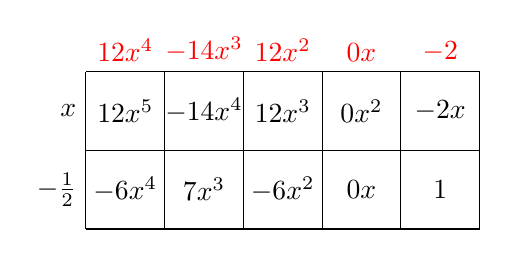
\begin{tikzpicture}
\draw (0,0) grid (5,2);
\node at (0,1.5) [left] {$x$};
\node at (0,0.5) [left] {$-\tfrac{1}{2}$};
\node at (0.5,1.5) {$12x^5$};
\onslide<2->{\node at (0.5,2) [above] {\color{red}$12x^4$};}
\onslide<3->{\node at (0.5,0.5) {$-6x^4$};}
\onslide<4->{\node at (1.5,1.5) {$-14x^4$};}
\onslide<5->{\node at (1.5,2) [above] {\color{red}$-14x^3$};}
\onslide<6->{\node at (1.5,0.5) {$7x^3$};}
\onslide<7->{\node at (2.5,1.5) {$12x^3$};}
\onslide<8->{\node at (2.5,2) [above] {\color{red}$12x^2$};}
\onslide<9->{\node at (2.5,0.5) {$-6x^2$};}
\onslide<10->{\node at (3.5,1.5) {$0x^2$};}
\onslide<11->{\node at (3.5,2) [above] {\color{red}$0x$};}
\onslide<12->{\node at (3.5,0.5) {$0x$};}
\onslide<13->{\node at (4.5,1.5) {$-2x$};}
\onslide<14->{\node at (4.5,2) [above] {\color{red}$-2$};}
\onslide<15->{\node at (4.5,0.5) {$1$};}
\end{tikzpicture}
\newline\\ \vspace{8pt}
\onslide<16->{
$12\left(\tfrac{1}{2}\right)^4 - 14\left(\tfrac{1}{2}\right)^3 + 12\left(\tfrac{1}{2}\right)^2 - 2 = 0$, \newline\\ so $x = -\tfrac{1}{2}$ has another root.}
\end{frame}

\begin{frame}{Example 4}
$12x^4 - 14x^3 + 12x^2 + 0x - 2$ \newline\\
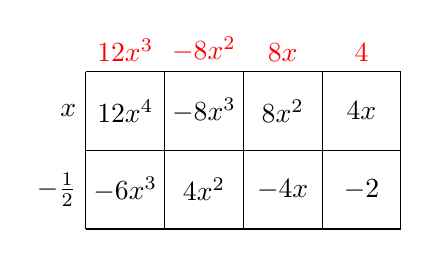
\begin{tikzpicture}
\draw (0,0) grid (4,2);
\node at (0,1.5) [left] {$x$};
\node at (0,0.5) [left] {$-\tfrac{1}{2}$};
\node at (0.5,1.5) {$12x^4$};
\onslide<2->{\node at (0.5,2) [above] {\color{red}$12x^3$};}
\onslide<3->{\node at (0.5,0.5) {$-6x^3$};}
\onslide<4->{\node at (1.5,1.5) {$-8x^3$};}
\onslide<5->{\node at (1.5,2) [above] {\color{red}$-8x^2$};}
\onslide<6->{\node at (1.5,0.5) {$4x^2$};}
\onslide<7->{\node at (2.5,1.5) {$8x^2$};}
\onslide<8->{\node at (2.5,2) [above] {\color{red}$8x$};}
\onslide<9->{\node at (2.5,0.5) {$-4x$};}
\onslide<10->{\node at (3.5,1.5) {$4x$};}
\onslide<11->{\node at (3.5,2) [above] {\color{red}$4$};}
\onslide<12->{\node at (3.5,0.5) {$-2$};}
\end{tikzpicture}
\\[12pt]

\onslide<13->{$12\left(\tfrac{1}{2}\right)^3 - 8\left(\tfrac{1}{2}\right)^2 + 8\left(\tfrac{1}{2}\right) + 4 \neq 0$} \newline\\
\onslide<14->{Now we can use the $x = -\tfrac{1}{3}$ rational zero.}
\end{frame}

\begin{frame}{Example 4}
$12x^3 - 8x^2 + 8x + 4$ \newline\\
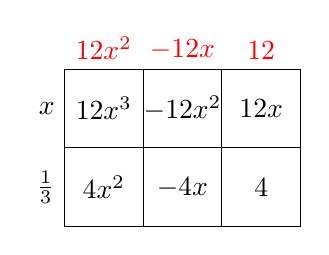
\begin{tikzpicture}
\draw (0,0) grid (3,2);
\node at (0,1.5) [left] {$x$};
\node at (0,0.5) [left] {$\tfrac{1}{3}$};
\node at (0.5,1.5) {$12x^3$};
\onslide<2->{\node at (0.5,2) [above] {\color{red}$12x^2$};}
\onslide<3->{\node at (0.5,0.5) {$4x^2$};}
\onslide<4->{\node at (1.5,1.5) {$-12x^2$};}
\onslide<5->{\node at (1.5,2) [above] {\color{red}$-12x$};}
\onslide<6->{\node at (1.5,0.5) {$-4x$};}
\onslide<7->{\node at (2.5,1.5) {$12x$};}
\onslide<8->{\node at (2.5,2) [above] {\color{red}$12$};}
\onslide<9->{\node at (2.5,0.5) {$4$};}
\end{tikzpicture}
\end{frame}

\begin{frame}{Example 4}
    \begin{align*}
        12x^2 - 12x + 12 &= 0 \\
        \onslide<2->{x^2 - x + 1 &= 0} \\[6pt]
        \onslide<3->{x &= \frac{1\pm \sqrt{1^2-4(1)(1)}}{2(1)}} \\[6pt]
        \onslide<4->{x &= \frac{1 \pm \sqrt{-3}}{2}} \\[6pt]
        \onslide<5->{x &= \frac{1 \pm i\sqrt{3}}{2}}
    \end{align*}
\onslide<6->{\[x = \frac{1}{2} \text{ (double root)}, \, -\frac{1}{3}, \, \frac{1}{2} \pm \frac{\sqrt{3}}{2}i\]}
\end{frame}

\end{document}
